% ============================================================
% sections/ch08-mrpt-mrci.tex —— 第 8 章 CASPT2/NEVPT2/MRCI
% 页数配额：5 页（±1）。数值只取自 data/h2m_pes.csv 与 data/ch4_results.csv。
% ============================================================

\section{CASPT2/NEVPT2/MRCI：如何给多参考态补动态相关？}
\label{ch:08:sec:title}

% ---- 1. 问题链 ----
\begin{problemchain}
\textbf{上一章留下的问题：}CASSCF 缺动态相关。\\
\textbf{本章为什么存在：}多参考微扰（CASPT2/NEVPT2）与 MRCI 在 CASSCF 参考上补动态相关。\\
\textbf{本章留下的新问题：}成本高、活性空间选择难。
\end{problemchain}

% ---- 2. 方法卡片 ----
\begin{methodcard}
\textbf{方法}：$n$ 电子价态微扰理论（NEVPT2），并与 CASPT2、MRCI 对照\quad
\textbf{文献}：\citep{andersson1990,angeli2001,werner1988,knowles1988,lischka2018mr}\\
\textbf{核心近似}：CASSCF 参考 + 二阶微扰（CASPT2/NEVPT2）或单双激发组态展开（MRCI）\\
\textbf{关键方程}：式~\eqref{ch:08:eq:pt2-energy}（二阶微扰能量）\\
\textbf{ORCA 关键词}：\texttt{! NEVPT2 def2-TZVPP TightSCF}，
并在 \texttt{\%casscf} 中写 \texttt{nel 8 norb 8 mult 1 nroots 1}\\
\textbf{成本标度}：$\mathcal{O}(N^5)$ 乘以活性空间因子\\
\textbf{能否变分 / 尺寸一致}：否 / 是（PT2）；MRCI 变分但不尺寸一致\\
\textbf{典型失效}：CASPT2 的入侵态、活性空间依赖、MRCI 的尺寸不一致
\end{methodcard}

% ---- 3. 正文 ----
\subsection{CASPT2：零阶 Hamiltonian 与有效 Hamiltonian}
\label{ch:08:sec:caspt2}

第 7 章的 CASSCF 把静态相关收进活性空间，但活性空间外的动态相关仍被丢掉。最直接的做法是以 CASSCF 波函数为零阶参考，对剩余的激发空间做二阶微扰，这就是 CASPT2\citep{andersson1990}。把 Hamiltonian 分成零阶与微扰两部分：
\begin{equation}
\op{H}=\op{H}_0+\op{V},
\qquad
\op{H}_0=\op{P}\op{F}\op{P}+\op{Q}\op{F}\op{Q},
\label{ch:08:eq:partition}
\end{equation}
其中 $\op{P}$ 是 CASSCF 参考态及其活性空间组态张成的模型空间，$\op{Q}=1-\op{P}$ 是正交补，$\op{F}$ 是广义 Fock 算符。式~\eqref{ch:08:eq:partition} 的关键在于零阶 Hamiltonian 用 Fock 算符而非完整的 $\op{H}$：这样 $\op{H}_0$ 在 $\op{P}$ 与 $\op{Q}$ 内可对角化，微扰展开才有可计算的分母。

在二阶微扰下，有效 Hamiltonian 可以写成
\begin{equation}
\op{H}_{\mathrm{eff}}^{(2)}
=\op{P}\op{H}\op{P}
+\op{P}\op{V}\op{Q}\,
\frac{1}{E_0-\op{H}_0}\,
\op{Q}\op{V}\op{P},
\label{ch:08:eq:caspt2-effective}
\end{equation}
其中 $E_0$ 是零阶能量。式~\eqref{ch:08:eq:caspt2-effective} 把 CASSCF 模型空间内的相互作用与外部激发空间的二阶反馈合在一起；对角化它，就得到 CASPT2 对各个态的修正。对基态，二阶能量修正可写成更熟悉的形式：
\begin{equation}
E^{(2)}
=\sum_{K\notin P}
\frac{\big|\bracket{\Phi_K|\op{V}|\Psi_0}\big|^2}
     {E_0-E_K},
\label{ch:08:eq:pt2-energy}
\end{equation}
其中 $\ket{\Psi_0}$ 是 CASSCF 参考态，$\ket{\Phi_K}$ 与 $E_K$ 是 $\op{H}_0$ 在 $\op{Q}$ 空间的本征态与本征值。式~\eqref{ch:08:eq:pt2-energy} 与 MP2 的式~\eqref{ch:04:eq:mp2-energy} 形式相同，区别在参考态：这里的分母不再是 HF 轨道能差，而是 CASSCF 零阶能量与外部组态能量之差。

CASPT2 最著名的失效是\textbf{入侵态}（intruder state）：当某个外部组态的能量 $E_K$ 与 $E_0$ 近简并时，式~\eqref{ch:08:eq:pt2-energy} 的分母趋于零，修正发散或给出错误符号。实际计算常用 level shift 或 IPEA shift 把分母推开，但 shift 的数值会改变结果，必须报告。另一个问题是活性空间依赖：换一个 CAS，参考态与 $\op{Q}$ 空间都变，CASPT2 能量也随之变；因此 CASPT2 不是“选了 CASSCF 就自动可靠”，活性空间仍需做收敛性检查。

\subsection{NEVPT2：Dyall Hamiltonian 与无入侵态}
\label{ch:08:sec:nevpt2}

NEVPT2 换一个零阶 Hamiltonian 来消除入侵态\citep{angeli2001}。它使用 Dyall Hamiltonian：
\begin{equation}
\op{H}_D
=\sum_{i}\varepsilon_i\,\op{a}_i^\dagger\op{a}_i
+\sum_{a}\varepsilon_a\,\op{a}_a^\dagger\op{a}_a
+\op{H}_{\mathrm{act}},
\label{ch:08:eq:dyall}
\end{equation}
其中 $i$ 取非活性轨道，$a$ 取虚轨道，$\op{H}_{\mathrm{act}}$ 是只用活性空间积分构造的 CAS Hamiltonian。式~\eqref{ch:08:eq:dyall} 把非活性与虚轨道写成简单的单体形式，把全部多体效应留在活性空间内。这样做的直接后果是：$\op{H}_D$ 的本征值由活性空间的激发能加上非活性/虚轨道的轨道能差组成，分母有一个与活性空间能隙同量级的下界，不会出现 CASPT2 那种任意小的入侵态分母。

NEVPT2 的二阶能量按外部组态相对参考态的“空穴/粒子”数分类：
\begin{equation}
E_{\mathrm{NEVPT2}}
=E_{\mathrm{CAS}}^{(0)}
+\sum_{l=1}^{8}\sum_{K\in Q_l}
\frac{\big|\bracket{\Phi_K|\op{V}|\Psi_0}\big|^2}
     {E_0^{(0)}-E_K^{(0)}},
\label{ch:08:eq:nevpt2-energy}
\end{equation}
其中 $Q_l$ 是第 $l$ 类外部组态（$0h$、$1h$、$2h$ 等，共八类）。式~\eqref{ch:08:eq:nevpt2-energy} 的每一类都可以用活性空间的低阶密度矩阵收缩，因而成本可控；同时因为 $\op{H}_D$ 的分母有下界，NEVPT2 对入侵态是“免疫”的。代价是 NEVPT2 对零阶 Hamiltonian 的选择更刚性：它不像 CASPT2 那样可以通过 shift 调节，活性空间选得不好时结果仍会偏，只是不会以发散的形式表现出来。

\subsection{MRCI 与 Davidson 校正}
\label{ch:08:sec:mrci}

MRCI 走另一条路：不做微扰，而是直接把参考态周围的单、双激发组态加进波函数\citep{werner1988,knowles1988,lischka2018mr}。多参考 CI 波函数写成
\begin{equation}
\ket{\Psi_{\mathrm{MRCI}}}
=\sum_{I} c_I\ket{\Phi_I},
\label{ch:08:eq:mrci-wavefunction}
\end{equation}
其中 $\ket{\Phi_I}$ 包括参考组态以及它们相对于参考空间的单、双激发；$\op{H}$ 在展开空间内对角化，CI 系数由本征值问题定出。式~\eqref{ch:08:eq:mrci-wavefunction} 的参考可以是多个 CASSCF 组态，因此它能同时描述静态相关与相当一部分动态相关。若把参考空间取成完整的 CAS，再把单、双激发加到所有参考组态上，就得到常用的 CAS+SD 型 MRCI；内部收缩（internally contracted）实现把激发组合并，显著降低维数。

MRCI 是变分的，但截断到单、双激发后不尺寸一致：两个远离的片段各自做 MRCI，再放在一起做超体系 MRCI，能量不能严格相加。Davidson 提出一个后验修正来估计缺失的高阶激发\citep{langhoff1974}：
\begin{equation}
E_{\mathrm{Davidson}}
=E_{\mathrm{MRCI}}
+\Big(1-\sum_{I\in\mathrm{ref}}|c_I|^2\Big)
 \big(E_{\mathrm{MRCI}}-E_{\mathrm{ref}}\big),
\label{ch:08:eq:davidson}
\end{equation}
其中 $\sum_{I\in\mathrm{ref}}|c_I|^2$ 是参考组态在 MRCI 波函数中的总权重，$E_{\mathrm{ref}}$ 是参考态能量。式~\eqref{ch:08:eq:davidson} 的括号衡量“参考态被激发组态稀释了多少”；稀释越多，修正越大。Davidson 校正能改善解离能等性质，但它不是严格的尺寸一致修正，不能把 MRCI+Q 当作尺寸一致方法。

尺寸一致性的差别可以写成一个简单判据。对两个无相互作用的片段 $A$、$B$，
\begin{equation}
E_{AB}(R\to\infty)=E_A+E_B
\label{ch:08:eq:size-consistency}
\end{equation}
是任何尺寸一致方法必须满足的条件。CASPT2 与 NEVPT2 在各自的 CASSCF 参考满足该条件时继承式~\eqref{ch:08:eq:size-consistency}；截断 MRCI 不满足，Davidson 校正只是把它向式~\eqref{ch:08:eq:size-consistency} 拉近，并不恢复严格等式。这一点与第 5 章 CISD 的病根相同：线性截断丢了断开激发，只是 MRCI 的参考空间更大、误差通常更小。

\subsection{CASPT2、NEVPT2 与 MRCI 的比较}
\label{ch:08:sec:compare}

三种方法的分工可以用表~\ref{ch:08:tab:compare} 概括。CASPT2 的零阶 Hamiltonian 最灵活，能通过 shift 处理入侵态，但 shift 与活性空间都会影响结果；NEVPT2 用 Dyall Hamiltonian 换来无入侵态与更好的尺寸行为，代价是零阶选择更刚性；MRCI 是变分的、能直接给出波函数，但截断后不尺寸一致，成本也更高。实际选择通常取决于体系大小、是否需要激发态/性质、以及活性空间能否可靠确定。

\begin{table}[t]
\centering
\small
\caption{多参考动态相关方法的比较。活性空间因子对所有方法都存在；MRCI 的参考空间越大，其组态数增长越快。}
\label{ch:08:tab:compare}
\begin{tabular}{@{}lcccc@{}}
\toprule
方法 & 零阶/展开 & 入侵态 & 变分 & 尺寸一致 \\
\midrule
CASPT2 & CASSCF + 广义 Fock & 有 & 否 & 是 \\
NEVPT2 & Dyall Hamiltonian & 无 & 否 & 是 \\
MRCI & 参考 + 单双激发 & 无 & 是 & 否（+Q 近似） \\
CCSD(T) & 单参考 + 微扰三激发 & 有 & 否 & 是 \\
\bottomrule
\end{tabular}
\end{table}

表~\ref{ch:08:tab:compare} 中的“无”与“有”不是绝对的精度排序。MRCI 变分且参考空间大，常被当作多参考基准；但它的尺寸不一致会在键断裂、弱相互作用中显现。CASPT2 与 NEVPT2 非变分，能量可能低于或高于精确值；NEVPT2 的无入侵态优势不等于它对活性空间不敏感。三者都需要在相同活性空间、相同基组下比较，不能把不同 CAS 的绝对能量混在一起。

\subsection{H$_2^-$ 势能曲线：CASSCF、NEVPT2 与 MRCI}
\label{ch:08:sec:h2m-mr}

图~\ref{ch:08:fig:h2m-mr} 把 H$_2^-$/def2-TZVPP 的 CASSCF(3,2)、NEVPT2 与 MRCI 绝对能量画在一起。三条曲线的最低点都在 1.2\,\AA{} 附近：CASSCF 为 $-0.985448$\,Eh，NEVPT2 为 $-1.020944$\,Eh，MRCI 为 $-1.034539$\,Eh。NEVPT2 在每个 R 上都低于 CASSCF，差值 0.0331--0.0391\,Eh；MRCI 又在每个 R 上都低于 NEVPT2，差值 0.0129--0.0137\,Eh。这正是第 7 章留下的“缺动态相关”被补上的直接证据：CASSCF 参考之上的修正不仅大，而且在整条曲线上稳定存在。

\begin{figure}[t]
\centering
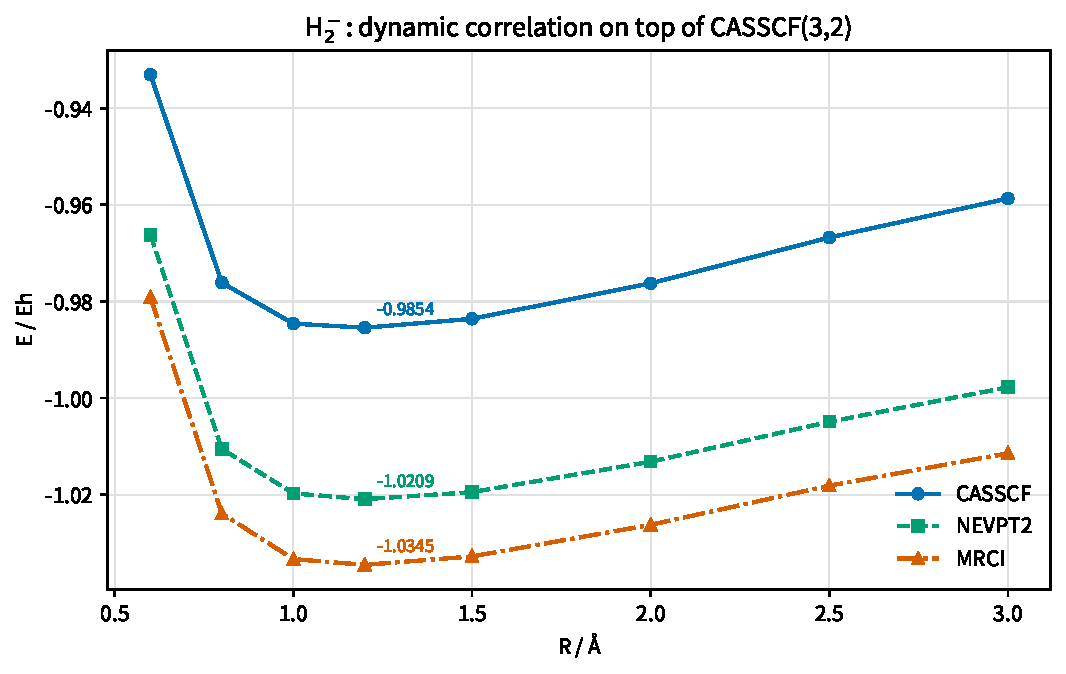
\includegraphics[width=0.86\textwidth]{figures/ch08/h2m_mr.pdf}
\caption{H$_2^-$/def2-TZVPP 的 CASSCF(3,2)、NEVPT2 与 MRCI 绝对能量（Eh）。
纵轴是绝对能量，因此可以直接看出三种方法在同一 R 上的相对位置；
三条曲线的最低点均在 $R=1.2$\,\AA{}。}
\label{ch:08:fig:h2m-mr}
\end{figure}

图~\ref{ch:08:fig:h2m-mr} 只画了三种方法，没有 CASPT2。原因不是 CASPT2 在物理上不适用，而是 ORCA 6.1.1 在 H$_2^-$/CAS(3,2) 的 CASPT2 清理阶段存在已知段错误\footnote{ORCA 6.1.1 在 H$_2^-$/CAS(3,2) 的 CASPT2 清理阶段存在已知段错误；本书因此不做 H$_2^-$ 的 CASPT2 扫描，CH$_4$ 的 CASPT2 数据来自 CAS(8,8) 计算。}。这是一个实现问题，不是 CASPT2 理论的失效；本书选择不伪造一条 CASPT2 曲线，而是用 NEVPT2 与 MRCI 展示多参考动态相关的效果。CASPT2 在 CH$_4$ 上的表现见下面的结果框。

\subsection{CH$_4$ 的 CAS(8,8) 结果与实现注记}
\label{ch:08:sec:ch4}

CH$_4$ 是弱静态相关体系，CAS(8,8) 的参考态已能描述其主要静态相关；在其上补动态相关，可以干净地比较三种方法。三种方法在 CH$_4$/def2-TZVPP 上给出的能量如下。CASPT2 为 $-40.420721$\,Eh，NEVPT2 为 $-40.405834$\,Eh，MRCI 为 $-40.428596$\,Eh；三者均低于 CASSCF 的 $-40.297163$\,Eh。MRCI 最低，CASPT2 次之，NEVPT2 再次；这与 H$_2^-$ 扫描中“NEVPT2 低于 CASSCF、MRCI 又低于 NEVPT2”的次序一致，说明动态相关修正的方向是稳定的。

但 CH$_4$ 的数值不能直接搬到 H$_2^-$ 上。H$_2^-$ 的 CAS(3,2) 是一个极小的活性空间，NEVPT2 与 MRCI 的修正主要来自活性空间外的动态相关；CH$_4$ 的 CAS(8,8) 已包含更多价相关，剩余修正较小。两者都说明 CASSCF 不是终点，但修正的绝对大小依赖活性空间。CASPT2 在 CH$_4$ 上能正常完成，正说明 8.5 节缺失的 H$_2^-$ CASPT2 曲线是 ORCA 对该特定体系/活性空间的清理 bug，而不是方法本身的普遍问题。

% ---- 4. CH4 结果框 ----
\begin{ch4box}
CH$_4$/def2-TZVPP：$E_{\mathrm{CASPT2}} = -40.420721$\,Eh
（CSV 精确值 $-40.420720703026$\,Eh），
$\Delta E = +11.22$\,kcal·mol$^{-1}$；
$E_{\mathrm{NEVPT2}} = -40.405834$\,Eh
（CSV 精确值 $-40.405833810464$\,Eh），
$\Delta E = +20.56$\,kcal·mol$^{-1}$；
$E_{\mathrm{MRCI}} = -40.428596$\,Eh
（CSV 精确值 $-40.428596004396$\,Eh），
$\Delta E = +6.28$\,kcal·mol$^{-1}$。
参考值为 CCSD(T) 的 $-40.438598$\,Eh。
在 CH$_4$ 上按能量从低到高为 MRCI、CASPT2、NEVPT2、CASSCF，
与 H$_2^-$ 扫描中 MRCI $<$ NEVPT2 $<$ CASSCF 的次序一致。
\end{ch4box}

% ---- 5. 常见陷阱 ----
\begin{pitfall}
\begin{itemize}
  \item \textbf{把 CASPT2 当作黑箱}：式~\eqref{ch:08:eq:pt2-energy} 的分母可能被入侵态击穿；level shift/IPEA shift 的取值会改变能量，必须与活性空间一起报告。
  \item \textbf{认为 NEVPT2 对活性空间不敏感}：Dyall Hamiltonian 只保证分母有下界，不保证结果与活性空间无关；式~\eqref{ch:08:eq:nevpt2-energy} 仍依赖 CAS 的选择。
  \item \textbf{把 MRCI 当尺寸一致方法}：MRCI 变分但不满足式~\eqref{ch:08:eq:size-consistency}；Davidson 校正式~\eqref{ch:08:eq:davidson} 只是近似补救，不是严格修正。
  \item \textbf{跨活性空间比较绝对能量}：CASPT2/NEVPT2/MRCI 的能量都建立在特定 CAS 上；换活性空间就是换参考态，绝对能量不可直接对比。
\end{itemize}
\end{pitfall}

% ---- 6. 小结 + 过渡 ----
\subsection*{小结}
CASPT2 用式~\eqref{ch:08:eq:caspt2-effective}--\eqref{ch:08:eq:pt2-energy} 在 CASSCF 参考上做二阶微扰，能补动态相关但受入侵态与 shift 影响；NEVPT2 用 Dyall Hamiltonian 式~\eqref{ch:08:eq:dyall} 消除入侵态，并按式~\eqref{ch:08:eq:nevpt2-energy} 分类求和；MRCI 用式~\eqref{ch:08:eq:mrci-wavefunction} 直接展开单双激发，变分但不尺寸一致，Davidson 校正只是近似。H$_2^-$ 扫描中 NEVPT2 与 MRCI 在每个 R 上都低于 CASSCF，CH$_4$ 上 MRCI 最低、CASPT2 次之、NEVPT2 再次、CASSCF 最高，二者共同说明多参考动态相关修正的方向稳定，但成本与活性空间选择仍是实际瓶颈。带着这个问题，我们进入第 9 章：DFT：能不能不写波函数？
